\section{Appendix}
\label{sec:appendix}

\begin{figure}[h!]
    \centering
    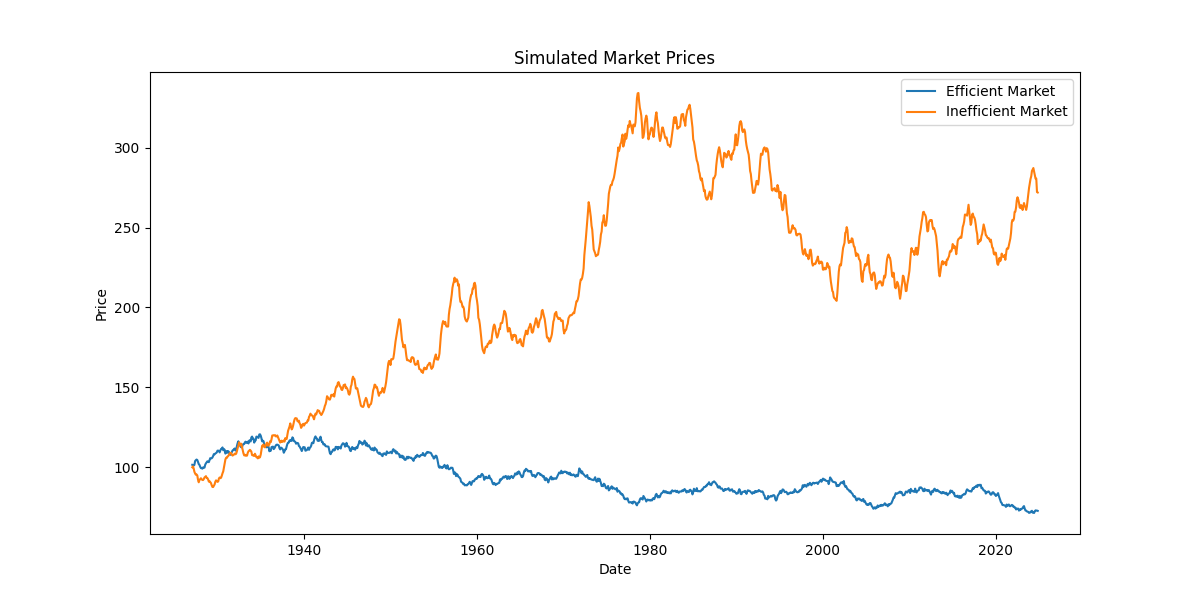
\includegraphics[width=0.8\textwidth]{../figs/Sample Simulated Market Prices.png}
    \caption{Simulated efficient and inefficient market prices. We generate a hundred of these price paths to show
    unbiasedness regression edge cases of perfectly efficient and inefficient markets.}
    \label{fig:sample_simulated_market}
\end{figure}

\subsection{Unbiasedness Regressions}
In this Appendix we build on the intuition behind the unbiasedness regressions and the measurement of market inefficiency using idealized results.
We provide plots from simulated efficient and inefficient markets, and show how the unbiasedness regressions can be used to measure the degree of inefficiency in the market.
Examples of efficient and inefficient market price paths are shown in Figure \ref{fig:sample_simulated_market}.

\subsubsection{Simulated Efficient Market}
\begin{equation}
    r_t \sim N(0, 0.1)
    \label{eq:simulated_efficient_market}
\end{equation}

In this section we simulate an efficient market, where returns are normally distributed with a mean of 0 and a standard deviation of 0.1.
They are independent random events, adhering to the strongest form of market efficiency (Equation~\ref{eq:simulated_efficient_market}).

\begin{figure}[h!]
    \centering
    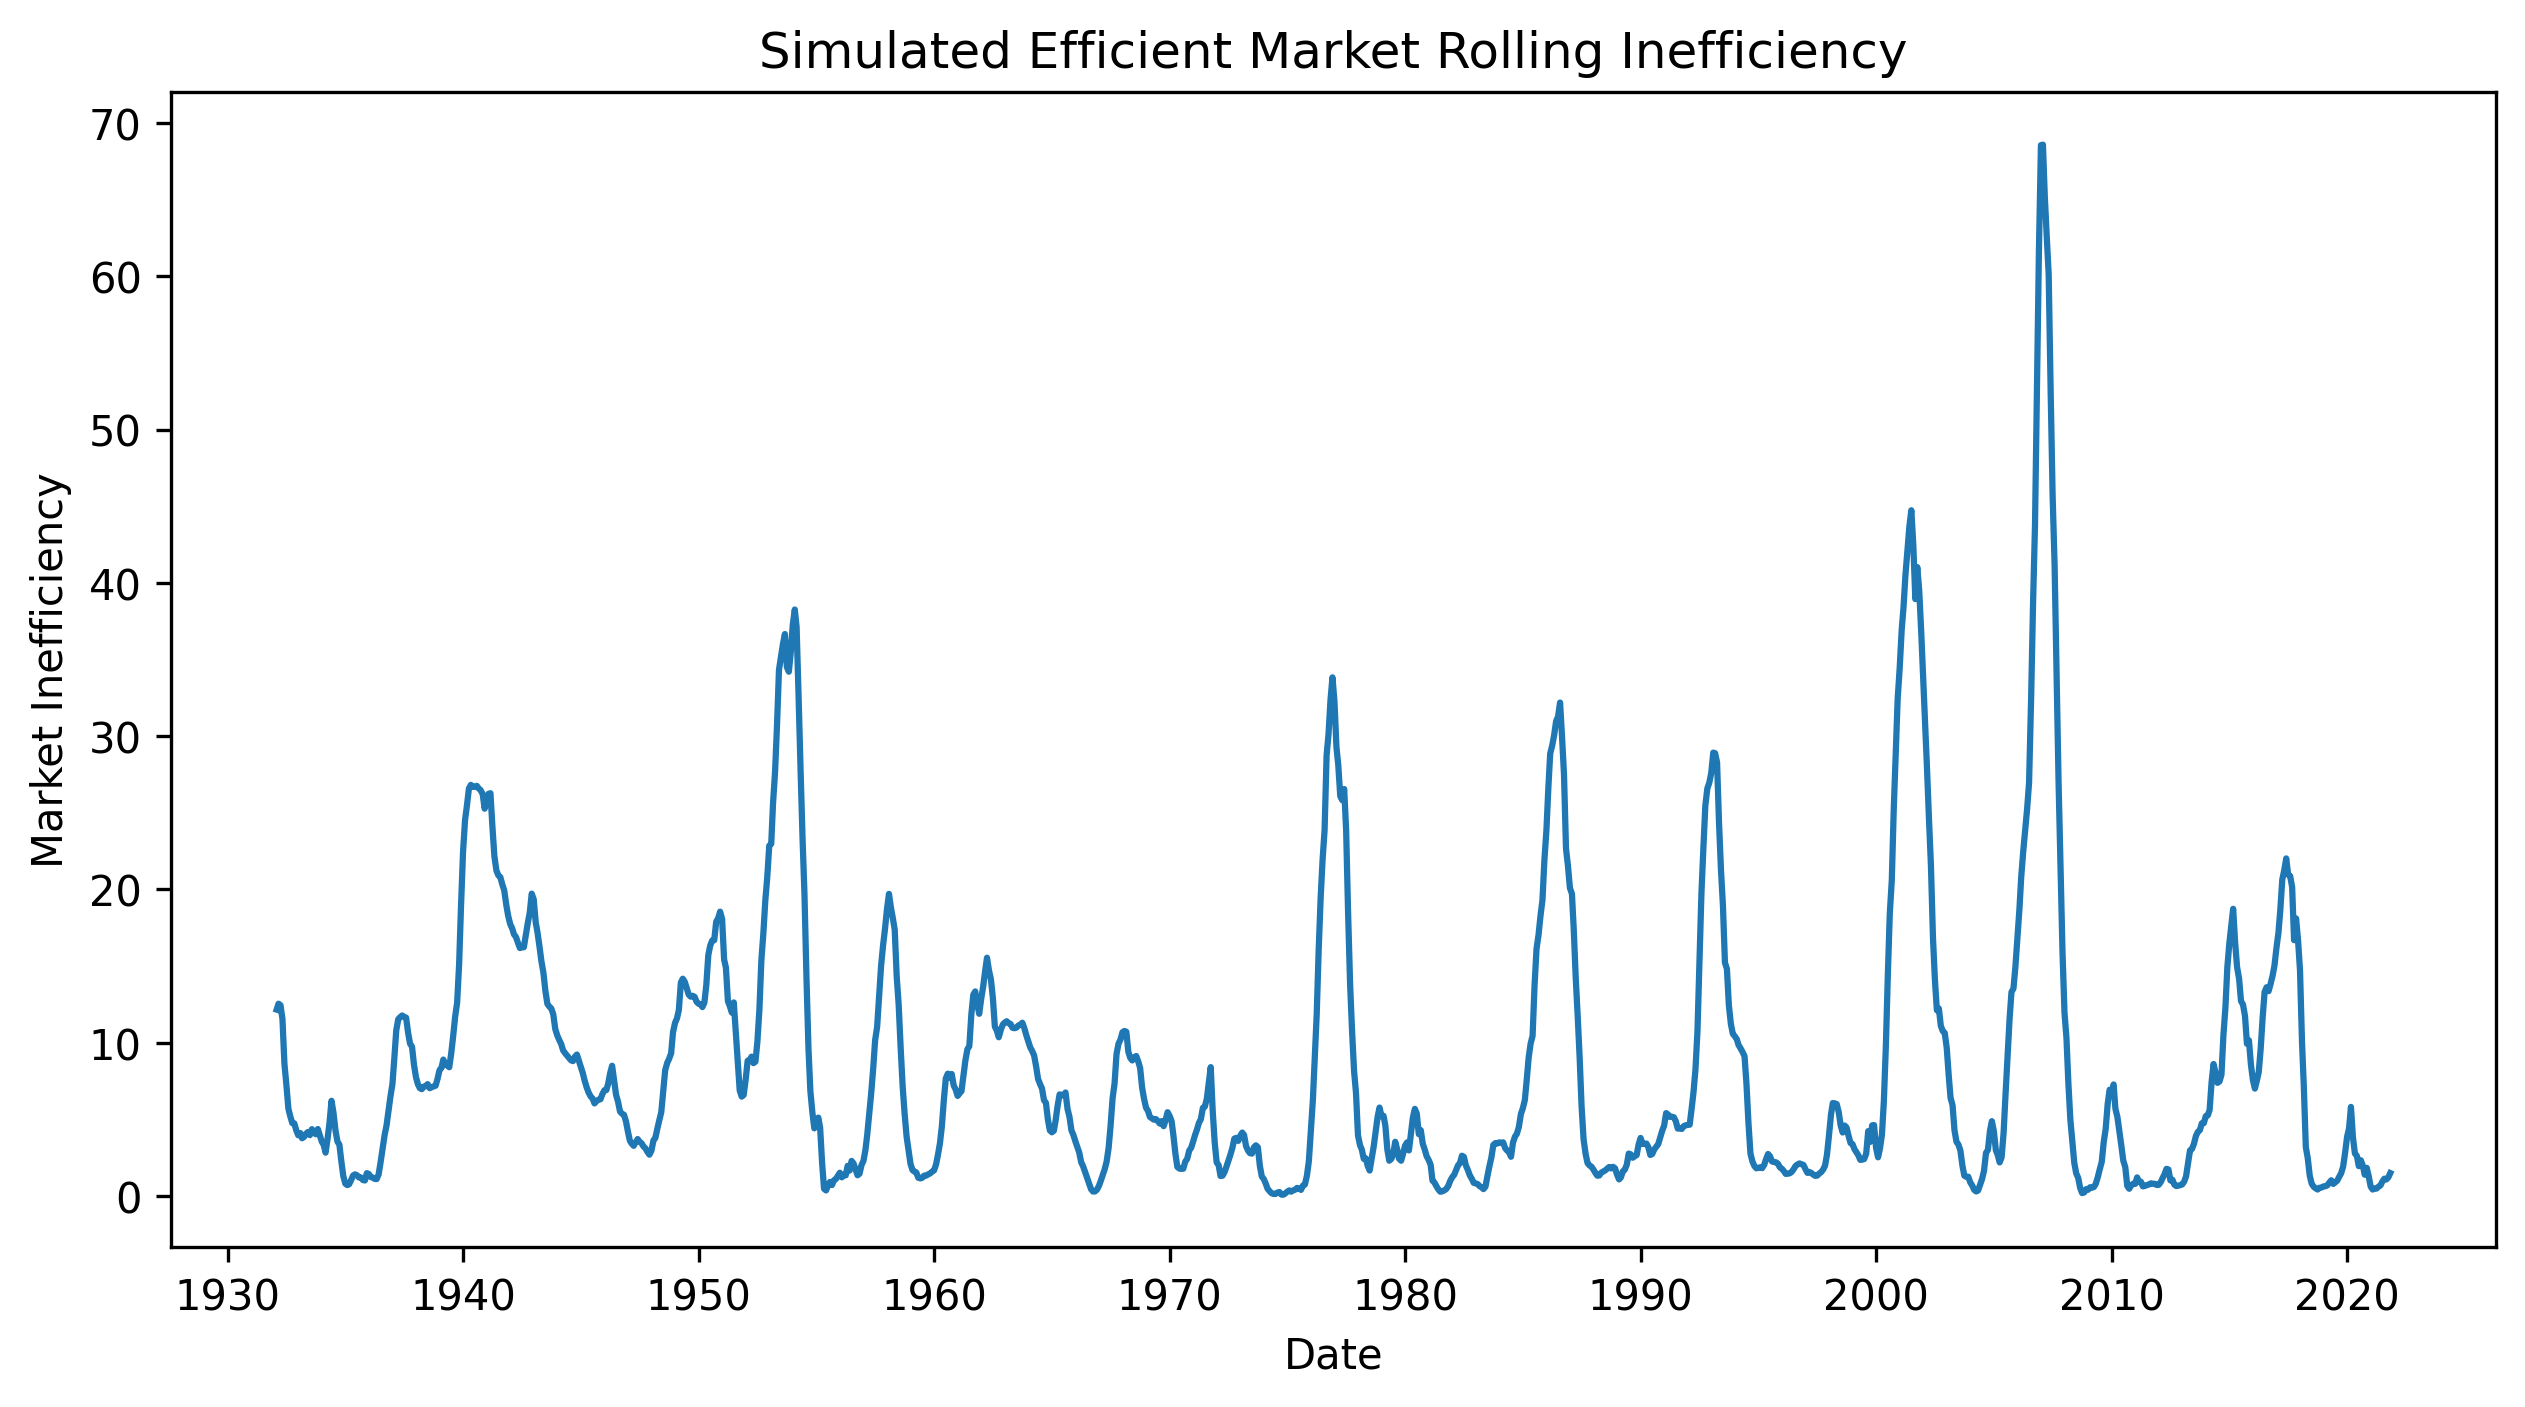
\includegraphics[width=0.8\textwidth]{../figs/Simulated Efficient Market Rolling Inefficiency.png}
    \caption{Rolling $Beta\_SSE$ scores on a simulated efficient market showing small spikes in inefficiency but reversion to the mean.}
    \label{fig:efficient_market}
\end{figure}

In Figure \ref{fig:efficient_market} we see the rolling inefficiency of the simulated efficient market.
Notice that the level remains low, with only small spikes in inefficiency.

We run a hundred possible price path simulations using the formula above, and present the unbiasedness regression results. 
What this shows us is the robustness of unbiasedness regressions. Since the market is simulated to be efficient, we expect the $\beta_t$ coefficients to be close to 1,
and the plot show us that this is the case.

\begin{figure}[h!]
    \centering
    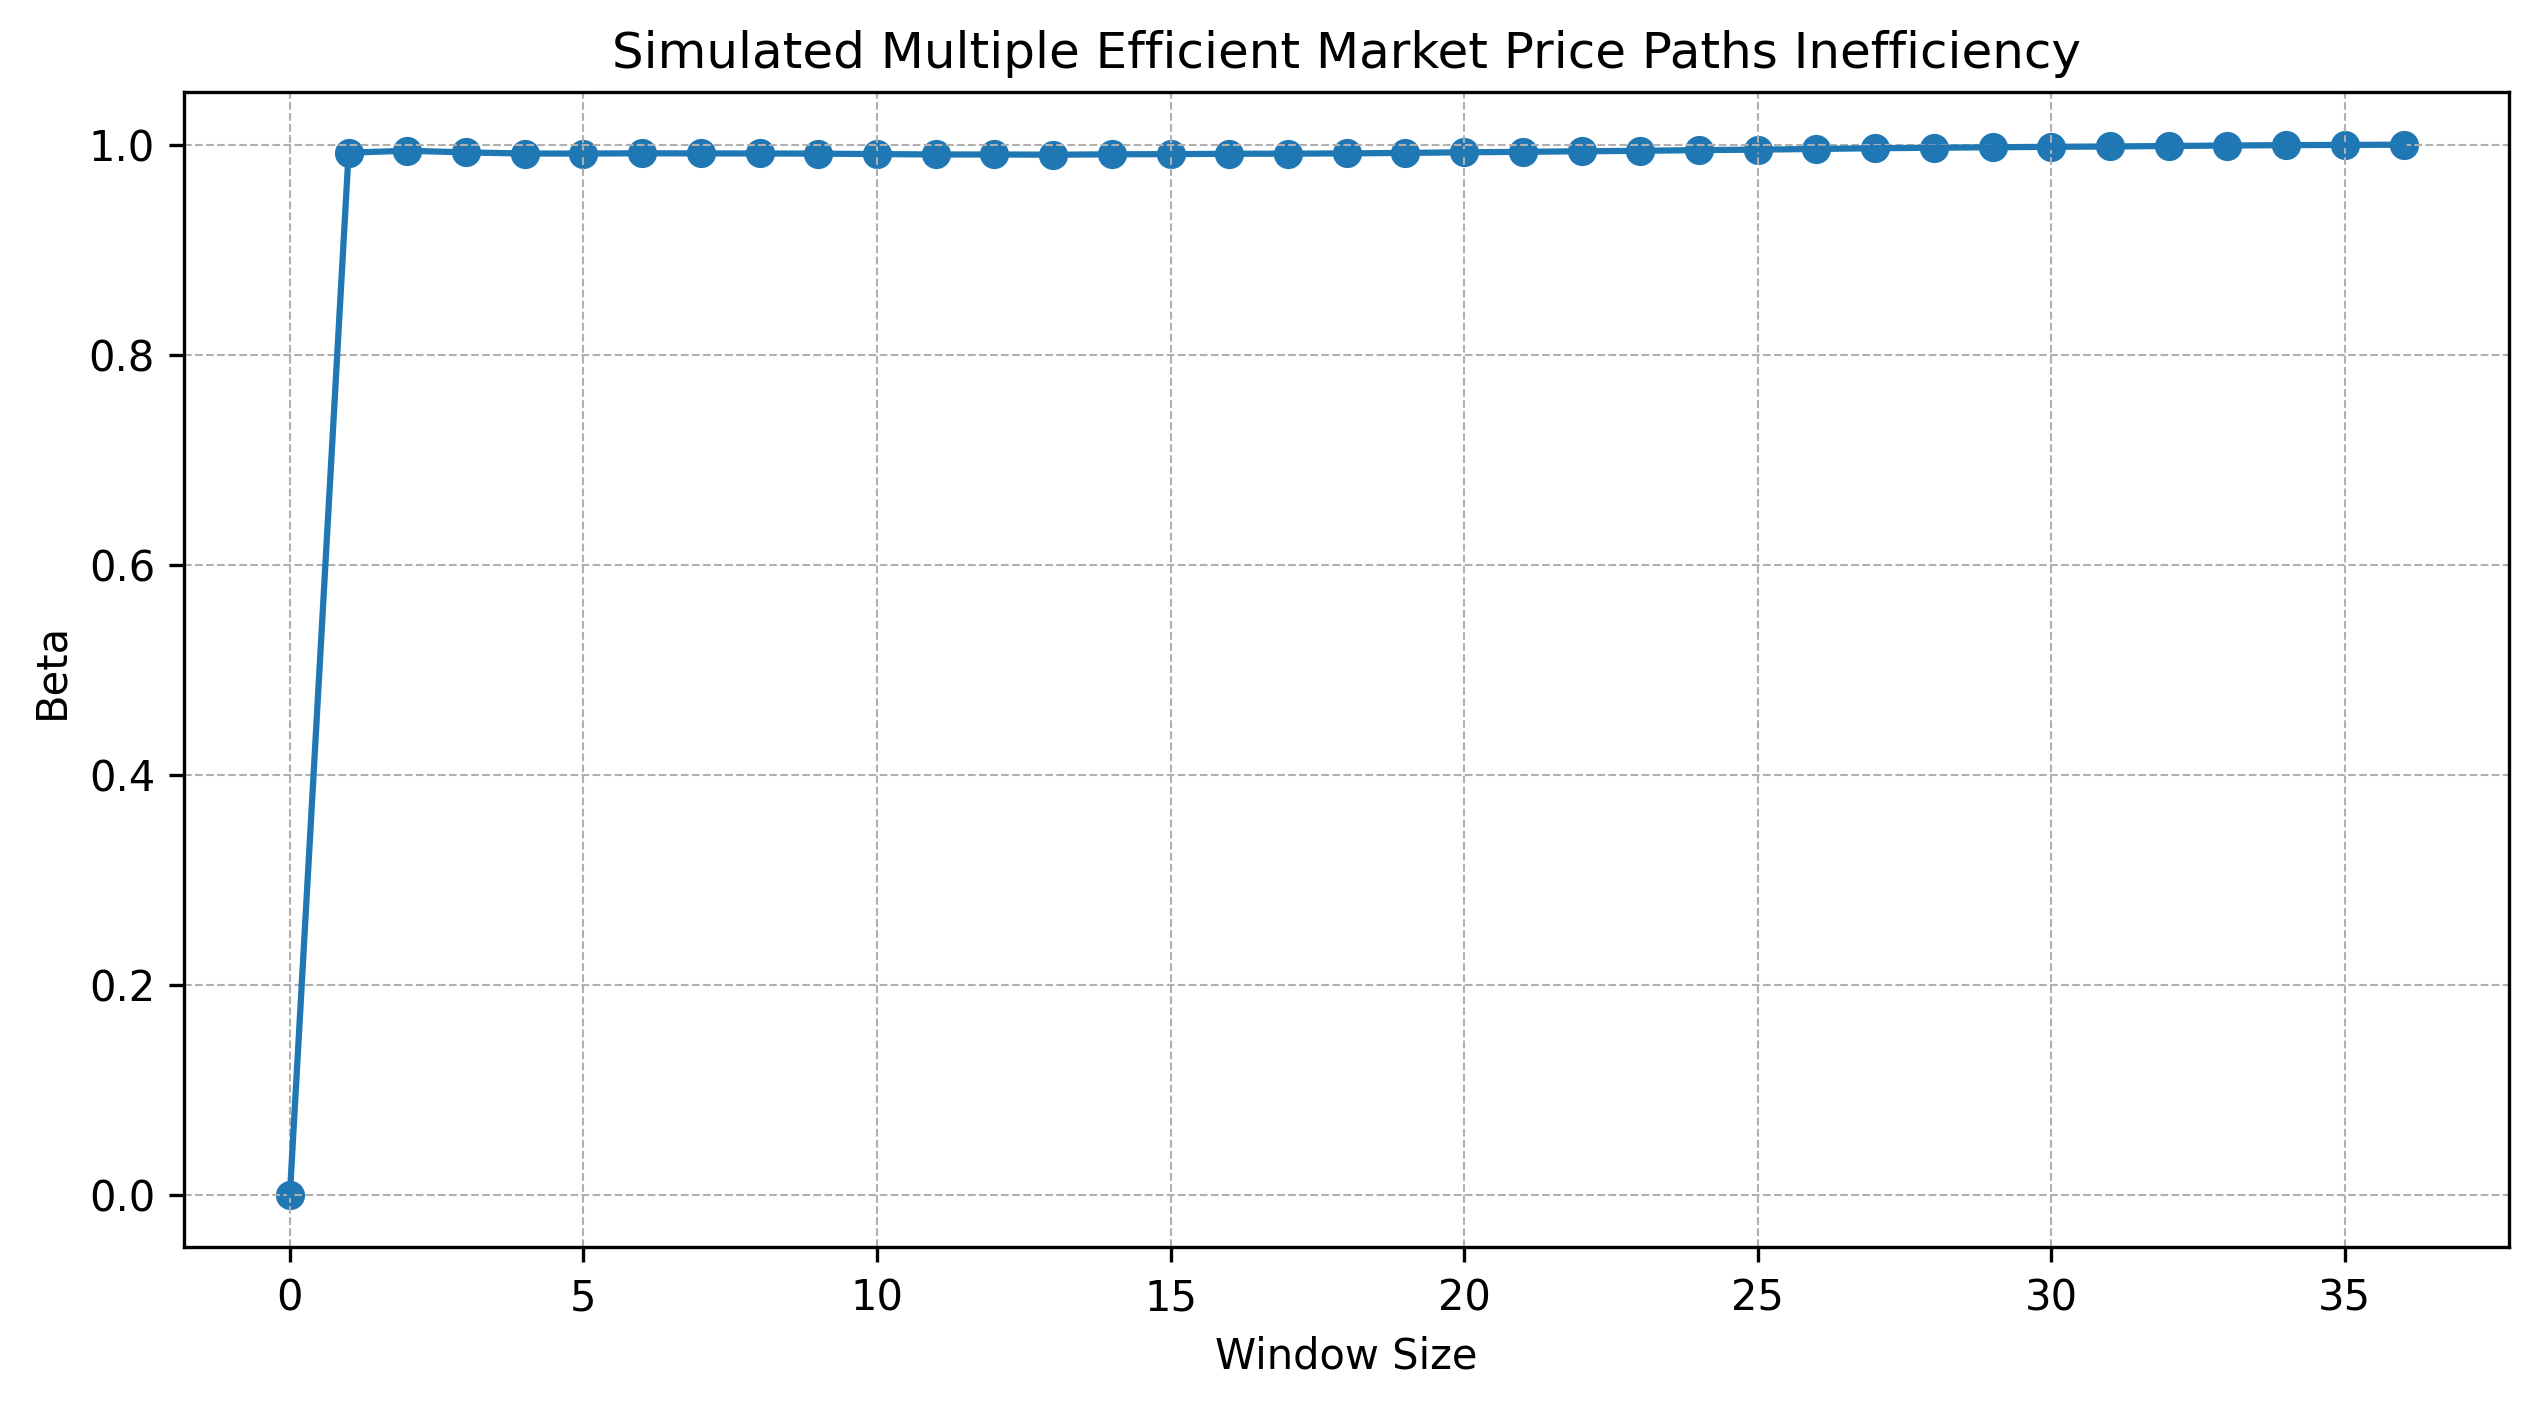
\includegraphics[width=0.8\textwidth]{../figs/Simulated Multiple Efficient Market Price Paths Inefficiency.png}
    \caption{An unbiasedness regression on a hundred simulated efficient price paths showing us that we should expect $\beta_t$ to be close to 1 in an efficient market.}
    \label{fig:efficient_market_unbiasedness}
\end{figure}

\subsubsection{Simulated Inefficient Market}
In this section we simulate an inefficient market, where returns are an AR(1) process (Equation~\ref{eq:simulated_inefficient_market}).:
\begin{equation}
    r_t = \phi r_{t-1} + \epsilon_t
    \label{eq:simulated_inefficient_market}
\end{equation}

where $\phi = 0.5$ and $\epsilon_t \sim N(0, 0.1)$. The resulting series of market inefficiency
 is shown in Figure \ref{fig:inefficient_market}. We see that there are much more frequent spikes of inefficiency, and the level of inefficiency is much higher than in the efficient market.

\begin{figure}[h!]
    \centering
    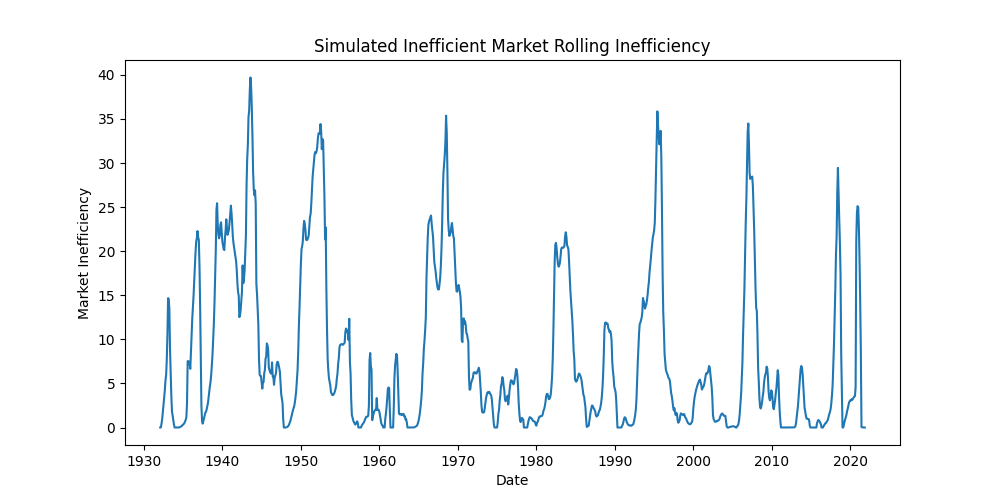
\includegraphics[width=0.8\textwidth]{../figs/Simulated Inefficient Market Rolling Inefficiency.png}
    \caption{Rolling $Beta\_SSE$ scores on a simulated inefficient market showing frequent and higher amplitude spikes in inefficiency.}
    \label{fig:inefficient_market}
\end{figure}

We run a hundred possible price path simulations using the framework above and present the unbiasedness regression results for an inefficient market.
We expect the $\beta_t$ coefficients to be generally further from 1, and the plot show us that this is the case.

\begin{figure}[h!]
    \centering
    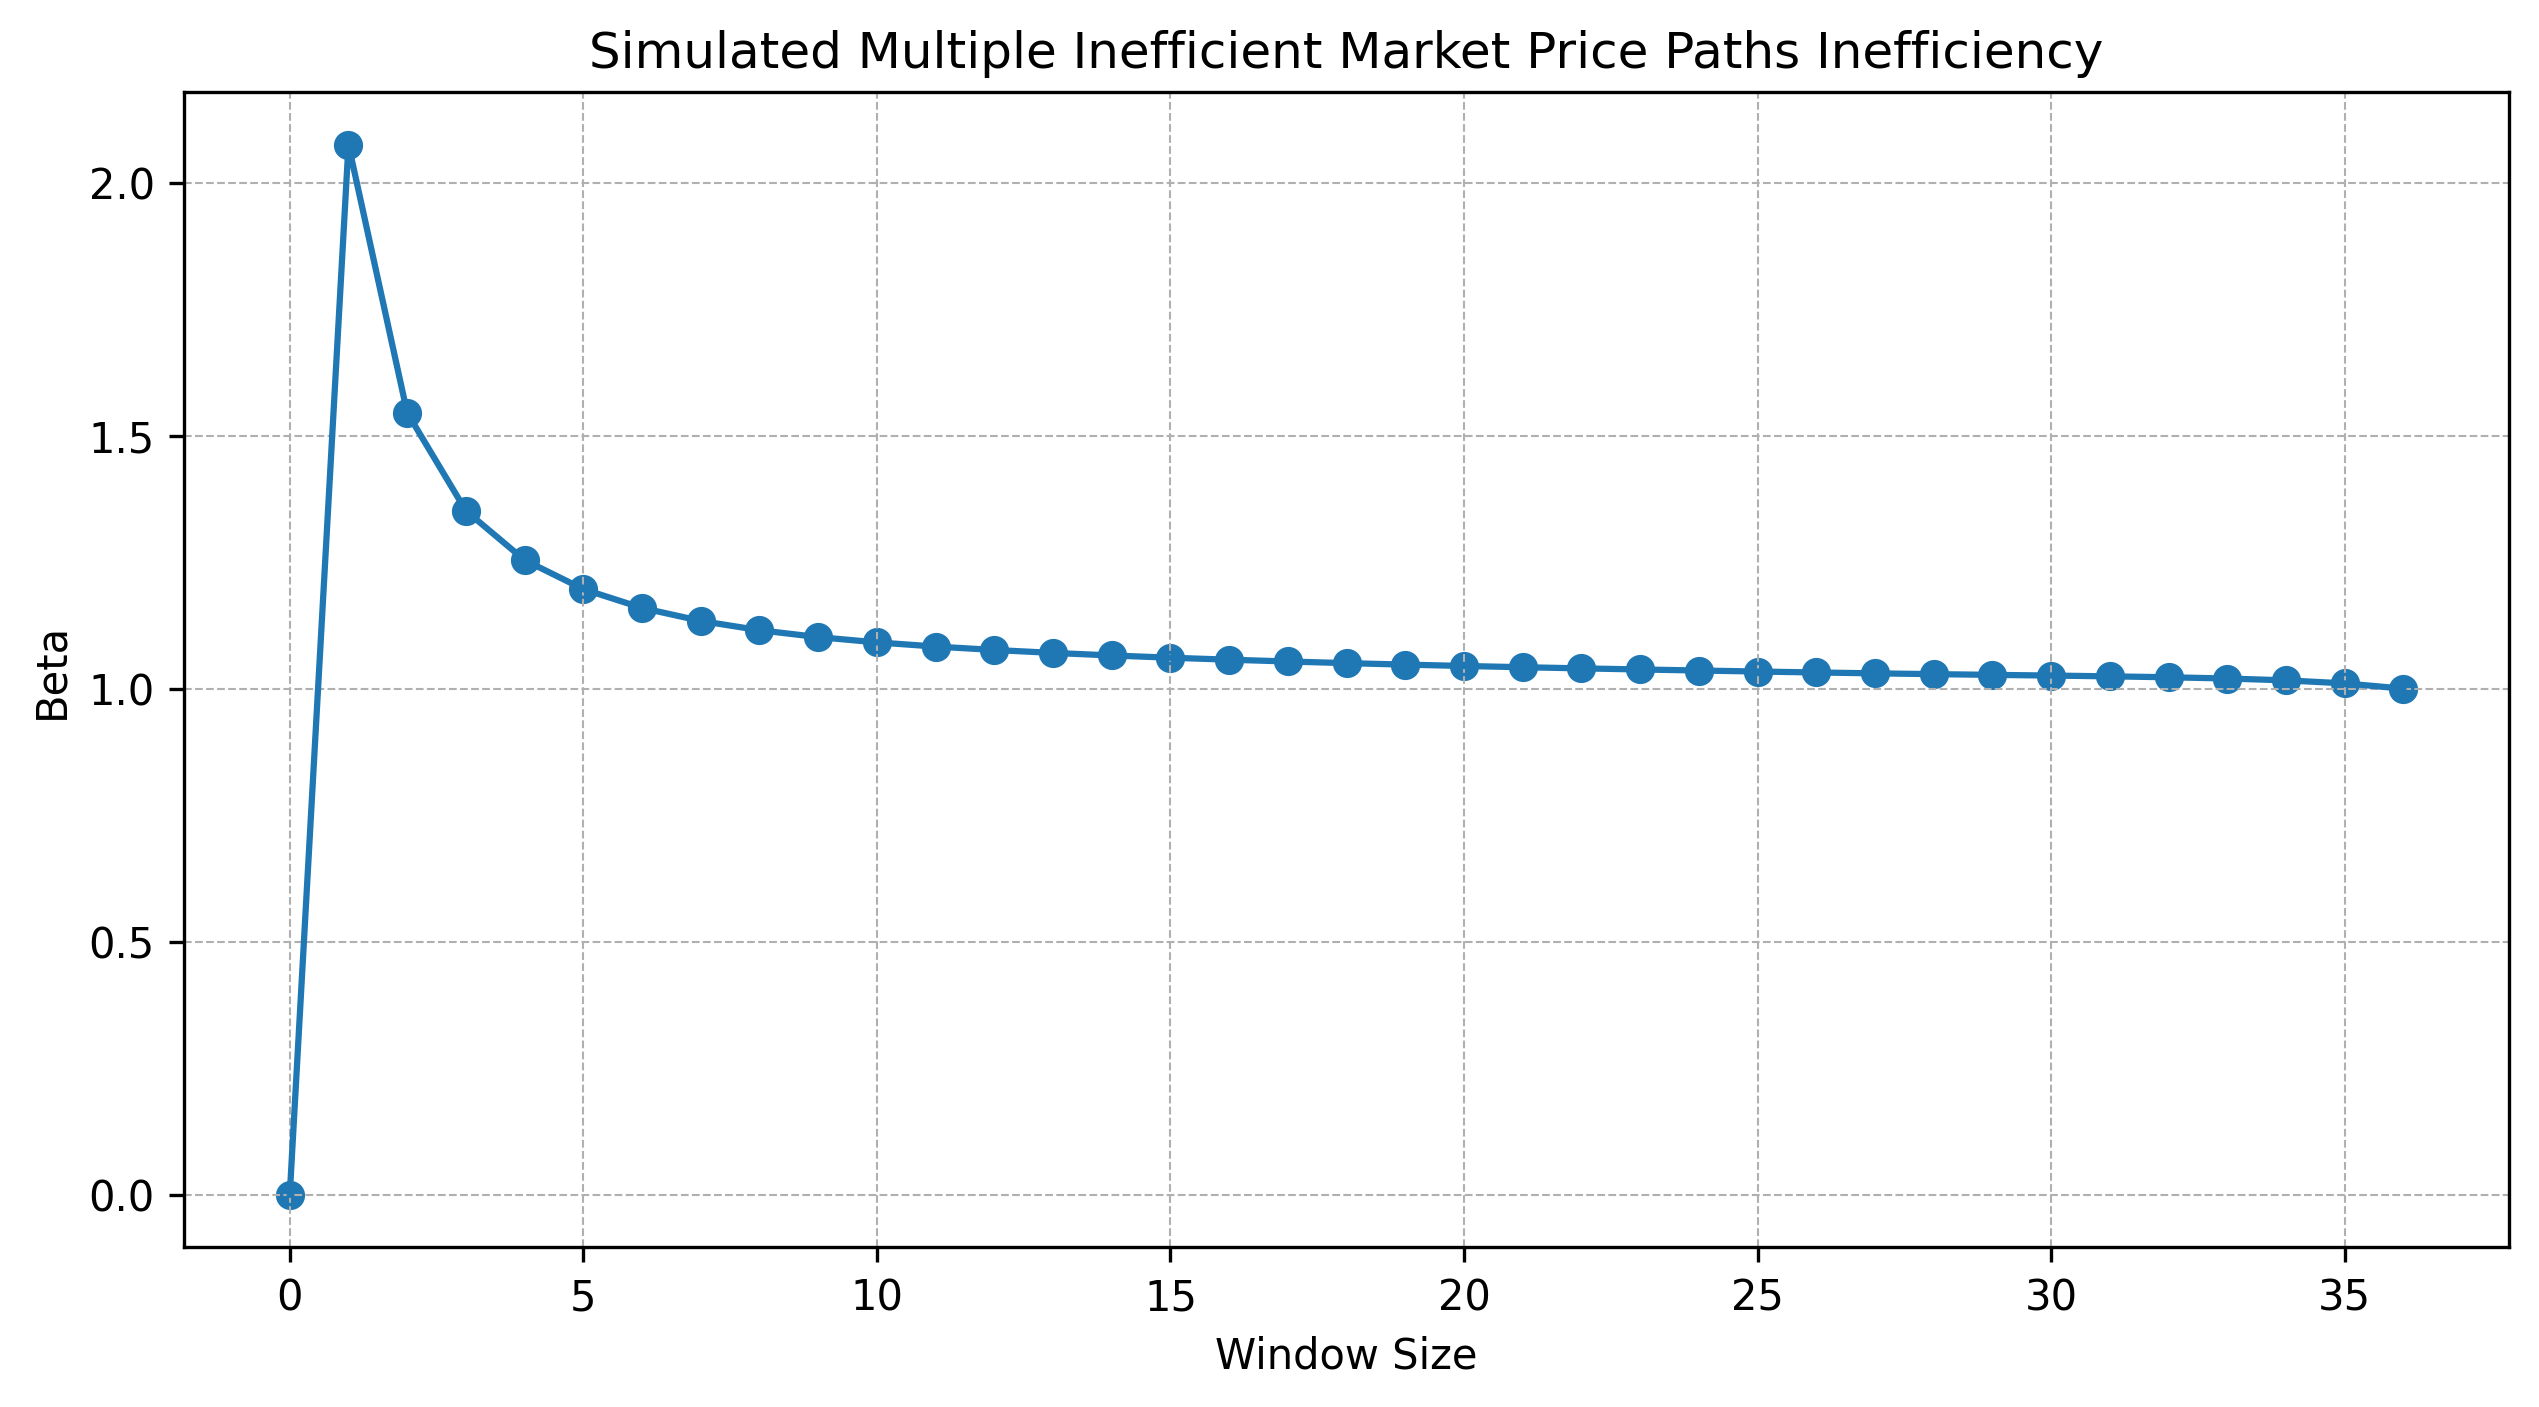
\includegraphics[width=0.8\textwidth]{../figs/Simulated Multiple Inefficient Market Price Paths Inefficiency.png}
    \caption{An unbiasedness regression on a hundred simulated inefficient price paths showing us that we should expect $\beta_t$ to be further from 1 in an inefficient market.}
    \label{fig:inefficient_market_unbiasedness}
\end{figure}

What these results tell us is that the unbiasedness regression is a robust tool for measuring market inefficiency, and our interpretation of the $\beta_t$ coefficients is consistent with empirical results.
Since these results are robust in the spot, our $Beta\_SSE$ score which generates a time series of these plots is also robust.